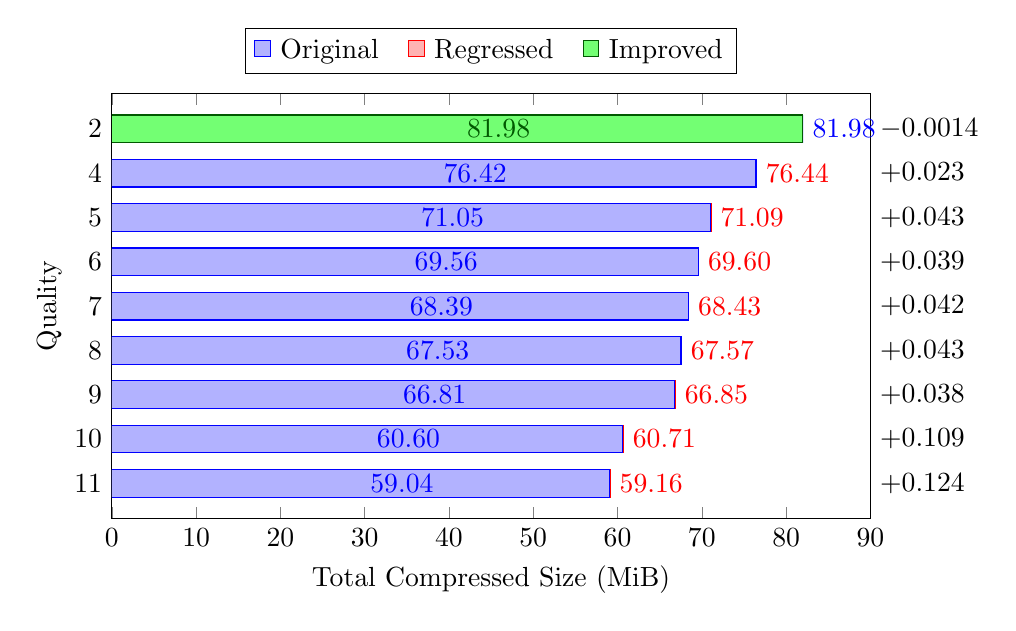
\begin{tikzpicture}
\begin{axis}[
	width = 0.925\textwidth,
	height = 0.96*\axisdefaultheight,
	xbar stacked,
	xmin = 0,
	xmax = 90,
	xtick distance = 10,
	y dir = reverse,
	ytick = data,
	ytick pos = left,
	yticklabels = {2, 4, 5, 6, 7, 8, 9, 10, 11},
	extra y ticks = {0, 1, 2, 3, 4, 5, 6, 7, 8},
	extra y tick labels = {$-0.0014$, $+0.023$, $+0.043$, $+0.039$, $+0.042$, $+0.043$, $+0.038$, $+0.109$, $+0.124$},
	extra y tick style = {ticklabel pos = right},
	scaled ticks = false,
	enlarge x limits = {abs = 0},
	enlarge y limits = {abs = 0.8},
	nodes near coords,
	nodes near coords align = {horizontal},
	nodes near coords style = {/pgf/number format/.cd, fixed zerofill, precision = 2},
	legend columns = -1,
	legend style = {
		at = {(0.5, 1.045)},
		anchor = south,
		column sep = 0.05cm,
		/tikz/every even column/.append style = {
			column sep = 0.3cm
		}
	},
	legend image code/.code = {
		\draw[#1] (0cm, -0.075cm) rectangle (0.2cm, 0.135cm);
	},
	xlabel = Total Compressed Size (MiB),
	ylabel = Quality,
	ylabel style = {yshift = -width(+0.0000)}
]
\legend{
	Original,
	Regressed,
	Improved
}
\addplot[blue, fill = blue!30!white] coordinates {
	(0, 0)
	(76.42, 1)
	(71.05, 2)
	(69.56, 3)
	(68.39, 4)
	(67.53, 5)
	(66.81, 6)
	(60.60, 7)
	(59.04, 8)
};
\addplot[red, fill = red!30!white, point meta = x] coordinates {
	(0, 0)
	(0.0230, 1)
	(0.0427, 2)
	(0.0394, 3)
	(0.0424, 4)
	(0.0429, 5)
	(0.0378, 6)
	(0.1093, 7)
	(0.1242, 8)
};
\addplot[green!35!black, fill = green!55!white] coordinates {
	(81.9786, 0)
};
\addplot[blue, fill = blue!30!white, point meta = x] coordinates {
	(0.0014, 0)
};
\end{axis}
\end{tikzpicture}